% !TeX root = ./ms.tex
\documentclass[modern]{aastex62}

% Load the corTeX style definitions
% !TeX root = ./ms.tex
% All the packages
\usepackage{url}
\usepackage{amsmath}
\usepackage{mathtools}
\usepackage{amssymb}
\usepackage{natbib}
\usepackage{graphicx}
\usepackage{calc}
\usepackage{etoolbox}
\usepackage{xspace}
\usepackage[T1]{fontenc} % https://tex.stackexchange.com/a/166791
\usepackage{textcomp}
\usepackage{ifxetex}
\ifxetex
  \usepackage{fontspec}
  \defaultfontfeatures{Extension = .otf}
\fi
\usepackage{fontawesome}
\usepackage{listings}
\usepackage{nicefrac}
\usepackage[bb=boondox]{mathalfa}
\usepackage{booktabs}
\usepackage{longtable}

% Shorthand for this paper
\newcommand{\starry}{\textsf{starry}\xspace}
\newcommand{\Python}{\textsf{Python}\xspace}
\newcommand{\cpp}{\textsf{C}++\xspace}
\newcommand{\bvec}[1]{{\ensuremath{\mathbf{#1}}}}
\newcommand{\xxx}[1]{{\color{red}#1}}
\DeclarePairedDelimiter\floor{\lfloor}{\rfloor}
\DeclarePairedDelimiter\ceil{\lceil}{\rceil}
\newcommand{\imag}{{\ensuremath{\mathbb{i}}}}
\newcommand{\quadquad}{\quad\quad\quad\quad}

\newcommand{\R}{\bvec{R}}
\newcommand{\AOne}{\bvec{A_1}}
\newcommand{\alm}{\bvec{a}}
\newcommand{\x}{\bvec{x}}
\newcommand{\D}{D}
\newcommand{\Doppler}{\bvec{D}}
\newcommand{\Surf}{\mathcal{S}}
\newcommand{\Curve}{\mathcal{C}}
\newcommand{\Dargs}{\bvec{d}}
\newcommand{\lmax}{\ensuremath{l_\mathrm{max}}}
\newcommand{\spot}{\texttt{SPOT}\xspace}
\newcommand{\vogtstar}{\texttt{VOGTSTAR}\xspace}
\newcommand{\kT}{\boldsymbol{\kappa}^\top}
\newcommand{\rhoT}{\boldsymbol{\rho}^\top}
\newcommand{\ylmbasis}{\boldsymbol{\psi}^\top}
\newcommand{\pbasis}{\boldsymbol{\phi}^\top}
\newcommand{\pbasisn}{\ensuremath{\phi_n}}
\newcommand{\azero}{\ensuremath{\bvec{a_0}}}

% References to text content
\newcommand{\documentname}{\textsl{article}}
\newcommand{\figureref}[1]{\ref{fig:#1}}
\newcommand{\Figure}[1]{Figure~\figureref{#1}}
\newcommand{\figurelabel}[1]{\label{fig:#1}}
\renewcommand{\eqref}[1]{\ref{eq:#1}}
\newcommand{\Eq}[1]{Equation~(\eqref{#1})}
\newcommand{\eq}[1]{\Eq{#1}}
\newcommand{\eqalt}[1]{Equation~\eqref{#1}}

% Add code, proof, and animation hyperlinks
\definecolor{linkcolor}{rgb}{0.1216,0.4667,0.7059}
\newcommand{\codeicon}{{\color{linkcolor}\faFileCodeO}}
\newcommand{\prooficon}{{\color{linkcolor}\faPencilSquareO}}
\newcommand{\codelink}[1]{\href{https://github.com/user/repo/blob/fe12fa16a5cc76c1ba72d97241fb9545da144edf/tex/figures/#1.py}{\codeicon}\,\,}
\newcommand{\animlink}[1]{\href{https://github.com/user/repo/blob/fe12fa16a5cc76c1ba72d97241fb9545da144edf/tex/figures/#1.gif}{\animicon}\,\,}
\newcommand{\prooflink}[1]{\href{https://github.com/user/repo/blob/fe12fa16a5cc76c1ba72d97241fb9545da144edf/tex/proofs/#1.ipynb}{\raisebox{-0.1em}{\prooficon}}}
\newcommand{\cilink}[1]{\href{https://dev.azure.com/user/repo/_build}{#1}}


% Define a proof environment for open source equation proofs
\newtagform{eqtag}[]{(}{)}
\newcommand{\currentlabel}{None}
\newenvironment{proof}[1]{%
  \ifstrempty{#1}{%
    \renewtagform{eqtag}[]{\raisebox{-0.1em}{{\color{red}\faPencilSquareO}}\,(}{)}%
  }{%
    \renewtagform{eqtag}[]{\prooflink{#1}\,(}{)}%
  }%
  \usetagform{eqtag}%
  \renewcommand{\currentlabel}{#1}
  \align%
}{%
  \endalign%
  \renewtagform{eqtag}[]{(}{)}%
  \usetagform{eqtag}%
  \message{<<<\currentlabel: \theequation>>>}%
}

% Display the runtime on Azure
\usepackage[skins]{tcolorbox}
\newtcbox{\figtimebox}{enhanced,nobeforeafter,tcbox raise=-0.8mm,boxrule=0.6pt,
  top=0.5mm,bottom=0mm,right=0mm,left=6mm,arc=1pt,boxsep=2pt,
  before upper={\vphantom{dlg}},colframe=linkcolor,coltext=linkcolor,
  fontupper=\sffamily\bfseries\tiny,colback=white,overlay={\begin{tcbclipinterior}
        \fill[linkcolor] (frame.south west)
        rectangle node[text=white,font=\sffamily\bfseries\tiny,rotate=0]{CPU}
        ([xshift=6mm]frame.north west);\end{tcbclipinterior}}}
\robustify{\figtimebox}
\pdfstringdefDisableCommands{%
  \def\figtimebox#1{'#1'}%
}
\newcommand{\figtime}[1]{\IfFileExists{figures/#1.py.time}%
  {%
    \cilink{\figtimebox{\input{figures/#1.py.time}\unskip s}}
  }{}}

% Define the `oscaption` command for open source figure captions
\newcommand{\oscaption}[2]{\caption{#2 \codelink{#1} \figtime{#1}}}

% Code examples
\definecolor{codegreen}{rgb}{0,0.6,0}
\definecolor{codegray}{rgb}{0.5,0.5,0.5}
\definecolor{codepurple}{rgb}{0.58,0,0.82}
\definecolor{backcolour}{rgb}{0.95,0.95,0.95}
\lstdefinestyle{mystyle}{
  backgroundcolor=\color{backcolour},
  commentstyle=\color{codegreen},
  keywordstyle=\color{magenta},
  numberstyle=\tiny\color{codegray},
  stringstyle=\color{codepurple},
  basicstyle=\small\ttfamily,
  breakatwhitespace=false,
  breaklines=true,
  captionpos=b,
  keepspaces=true,
  numbers=left,
  numbersep=5pt,
  showspaces=false,
  showstringspaces=false,
  showtabs=false,
  tabsize=2,
  aboveskip=1em,
  belowskip=1em,
  keywords=[2]{map},
  keywordstyle=[2]{\color{black!80!black}},
  upquote=true
}
\lstset{style=mystyle}

% Typography obsessions
\setlength{\parindent}{3.0ex}
\renewcommand\quad{\hskip\fontdimen3\font}

% https://tex.stackexchange.com/a/184474
\usepackage{stackengine,scalerel}
\def\lnlam{\ThisStyle{\ensurestackMath{\stackon[-2.4\LMpt]{%
        \SavedStyle\lambda}{\kern-.5pt\kern\LMpt\rule{1\LMex}{.25pt+.15\LMpt}}}}}

% Shorthand for this paper
\usepackage{xifthen}
\newcommand{\dd}{\ensuremath{\mathrm{d}}}
\newcommand{\STARRYQUADPOINTS}{100\xspace}
\newcommand{\bkappa}{\boldsymbol{\kappa}}
\newcommand{\blambda}{\boldsymbol{\lambda}}
\newcommand{\bxi}{\boldsymbol{\xi}}
\newcommand{\vmax}{{v_\mathrm{max}}}
\newcommand{\kapint}[1]{%
\sum_{i = 0}^{\frac{N - 1}{2}}
\int\limits_{\frac{1}{2}\kappa_{2i}}^{\frac{1}{2}\kappa_{2i+1}}
#1
\dd\varphi
}
\newcommand{\lamint}[1]{%
\sum_{i = 0}^{\frac{N - 1}{2}}
\int\limits_{\frac{1}{2}\lambda_{2i}}^{\frac{1}{2}\lambda_{2i+1}}
#1
\dd\varphi
}
\newcommand{\coshalfkap}[1][]{%
\ifthenelse{%
    \equal{#1}{}
}{
    \cos\left(\frac{\bkappa}{2}\right)
}{
    \cos^{#1}\left(\frac{\bkappa}{2}\right)
}}
\newcommand{\sinhalfkap}[1][]{%
\ifthenelse{%
    \equal{#1}{}
}{
    \sin\left(\frac{\bkappa}{2}\right)
}{
    \sin^{#1}\left(\frac{\bkappa}{2}\right)
}}
\newcommand{\DE}{\Delta \boldsymbol{E}(k^2, \bkappa)}
\newcommand{\DF}{\Delta \boldsymbol{F}(k^2, \bkappa)}
\newcommand{\sgn}{{\mathrm{sgn}}}
\newcommand{\xhat}{\ensuremath{\mathbf{\hat{x}}}\xspace}
\newcommand{\yhat}{\ensuremath{\mathbf{\hat{y}}}\xspace}
\newcommand{\zhat}{\ensuremath{\mathbf{\hat{z}}}\xspace}


% Bibliography stuff
\bibliographystyle{aasjournal}

% Begin!
\begin{document}

% Title
\title{Occultation Light Curves in Reflected Light}

% Author list
\author[0000-0002-0296-3826]{Rodrigo Luger}
\email{rluger@flatironinstitute.org}
\affil{Center~for~Computational~Astrophysics, Flatiron~Institute, New~York, NY}
%

\begin{abstract}
    Abstract here.
    %
    \href{https://github.com/rodluger/starrynight}{\color{linkcolor}\faGithub}
\end{abstract}

%
\section{Introduction}
\label{sec:intro}
%
This is an extension of \citet{Luger2019}.

\pagebreak

%
\section{The Problem}
\label{sec:the-problem}
%
As in \citet{Luger2019}, we compute the instantaneous visible flux $f$ from
a spherical body whose surface intensity is described by the spherical harmonic
coefficient vector $\mathbf{y}$ in some static frame $\mathcal{F}$ as
%
\begin{align}
    \label{eq:sTARRy}
    f = \bvec{s}^\top \bvec{A} \bvec{R}' \bvec{R} \bvec{y}
    \quad,
\end{align}
%
where $\bvec{R}$ and $\bvec{R}'$ are spherical harmonic rotation matrices
\citep[\S3.3 of][]{Luger2019},
$\bvec{A}$ is the change-of-basis matrix from spherical harmonics
to a basis $\tilde{\bvec{g}}$ \citep[Equation B13 in][]{Luger2019},
and $\bvec{s}^\top$ is the \emph{solution vector}, the integral of each
of the basis functions in $\tilde{\bvec{g}}$ over
the projected visible disk of the body (which may be partially occulted by
another spherical body).
%
The basis $\tilde{\bvec{g}}$ is called the \emph{Green's basis}; its name
stems from the fact that its components have a structure that makes integration
by Green's theorem convenient. Its components were defined in
Equation~11 of \citet{Luger2019b}:
%
\begin{proof}{bg}
    \tilde{g}_{l,m} &=
    \begin{dcases}
        %
        \frac{\mu+2}{2}x^\frac{\mu}{2} y^\frac{\nu}{2}
         & \qquad \mu, \nu \, \mathrm{even}
        \\[1em]
        %
        z(x, y)
         & \qquad \mu = \nu = 1
        \\[1em]
        %
        3x^{l-2}yz(x, y)
         & \qquad \nu \, \mathrm{odd}, \,
        \mu = 1, \,
        \frac{\mu + \nu}{2} \, \mathrm{even}
        \\[1em]
        %
        z(x, y)
        \bigg(
        -x^{l-3} + x^{l-1} + 4x^{l-3}y^2
        \bigg)
         & \qquad \nu \, \mathrm{odd}, \,
        \mu = 1, \,
        \, \mathrm{odd}
        \\[1em]
        %
        z(x, y)
        \bigg(
        \frac{\mu-3}{2} x^\frac{\mu-5}{2} y^\frac{\nu-1}{2}
        \ - \
        \frac{\mu-3}{2} x^\frac{\mu-5}{2} y^\frac{\nu+3}{2}
        \\
        \qquad\qquad \ - \
        \frac{\mu+3}{2} x^\frac{\mu-1}{2} y^\frac{\nu-1}{2}
        \bigg)
         & \qquad \mathrm{otherwise}
        \quad,
    \end{dcases}
    \label{eq:bg}
\end{proof}
%
where $x$ and $y$ are the Cartesian coordinates on the surface
of the projected
disk of the body, with $z(x, y) = \sqrt{1 - x^2 - y^2}$, and
%
\begin{align}
    \label{eq:munu}
    \mu & = l - m
    \nonumber     \\
    \nu & = l + m
    \quad.
\end{align}
%
The vector $\tilde{\bvec{g}}$ is ordered such that
the component at index $n$ is $\tilde{g}_{l,m}$, with
\begin{align}
    \label{eq:lm}
    l & = \floor*{\sqrt{n}} \nonumber \\
    m & = n - l^2 - l
    \quad.
\end{align}
Finally, the rotation matrix $\bvec{R} = \bvec{R}(i, \lambda, \theta)$
rotates the body to the correct orientation on the sky given its
inclination $i$, obliquity $\lambda$, and rotational phase $\theta$,
while $\bvec{R}'$ rotates the body on the plane
of the sky into the frame $\mathcal{F}'$ in which the integration is
actually performed, with the occultor along the $+y$-axis.
For more information on all of these terms, the reader is referred to
\citet{Luger2019}.

\begin{figure}[t!]
    \begin{centering}
        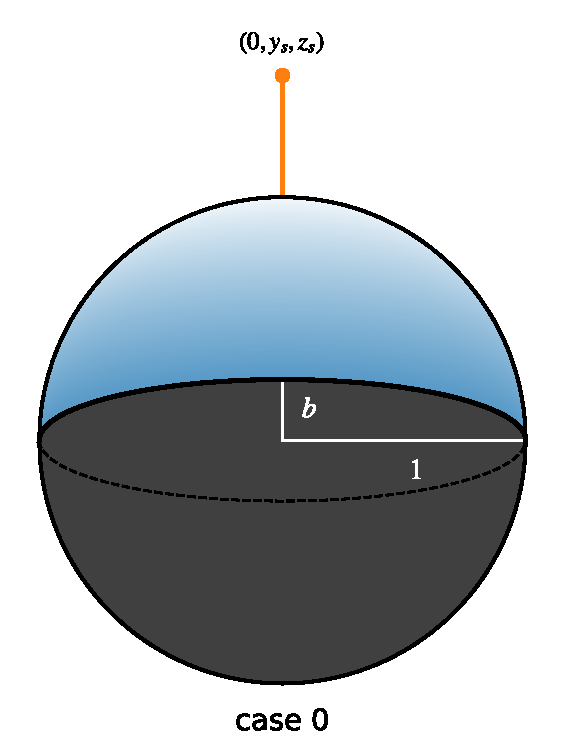
\includegraphics[width=0.35\linewidth]{figures/illum.pdf}
        \oscaption{illum}{%
            Illumination geometry for the unocculted case.
            A point source at Cartesian coordinates
            $(0, y_s, z_s)$ illuminates a uniform,
            Lambertian, spherical body of radius unity. The observed
            radiance falls off as the cosine of the angle $\phi$ between the
            source and the surface normal. Beyond the terminator
            (defined by $\phi = \frac{\pi}{2}$), the radiance is zero. In
            projection, the terminator is a segment of an ellipse of semi-major
            axis unity and semi-minor axis
            $b = -\nicefrac{z_s}{\sqrt{y_s^2 + z_s^2}}$.
            \label{fig:illum}
        }
    \end{centering}
\end{figure}

The derivations in \citet{Luger2019} assume that the coefficient vector
$\mathbf{y}$ describes the \emph{emissivity} of the body, which (in the
absence of limb darkening) is assumed to be Lambertian, i.e., all points on the
surface emit equally in all directions.
Here, we derive the solution to the occultation problem for Lambertian
reflectance, in which case the vector $\mathbf{y}$ describes the
surface \emph{reflectivity} (or \emph{Bond albedo}). Specifically, we assume
the body is illuminated by a point-like source and the radiance at any point
is proportional to the cosine of the angle $\phi$ between the incident light
and the surface normal. Points for which $\phi \ge \frac{\pi}{2}$ are
unilluminated and therefore have radiance of zero; see Figure~\ref{fig:illum}.

In \citet{Luger2019}, the crux of the problem was to compute the terms in the
vector $\bvec{s}^\top$, which are surface integrals over
the region of the occulted body that is visible to
the observer (Figure 2 in that paper). Here, these integrals are significantly
more difficult, because they involve not only the intersection of the
limbs of the two bodies, but also intersections with the elliptical
day/night terminator of the occulted body. Figure~\ref{fig:cases} shows the
eight families of cases involving an occultation of an illuminated body by
a spherical occultor. Each of these cases correspond to distinct ways in
which the limb of the occultor can intersect with the limb of the occulted
body and its terminator; together, these cases encompass all possible
occultation configurations, for any illumination angle, occultor size, and
occultor position. In the next three sections, we present the solution for the
$\bvec{s}^\top$, and hence for the total visible flux, for each of these cases.

% case 0: sTr
% case 1: 0
% case 2: sTr
% case 3: sTe * I + ~sTr
% case 4: sTe * I
% case 5: sTr - sT0 * I
% case 6: (sTe + sT0) * I + ~sTr
% case 7: (sTe - sT0) * I
% case 8: sT0 * I

\begin{figure}[t!]
    \begin{centering}
        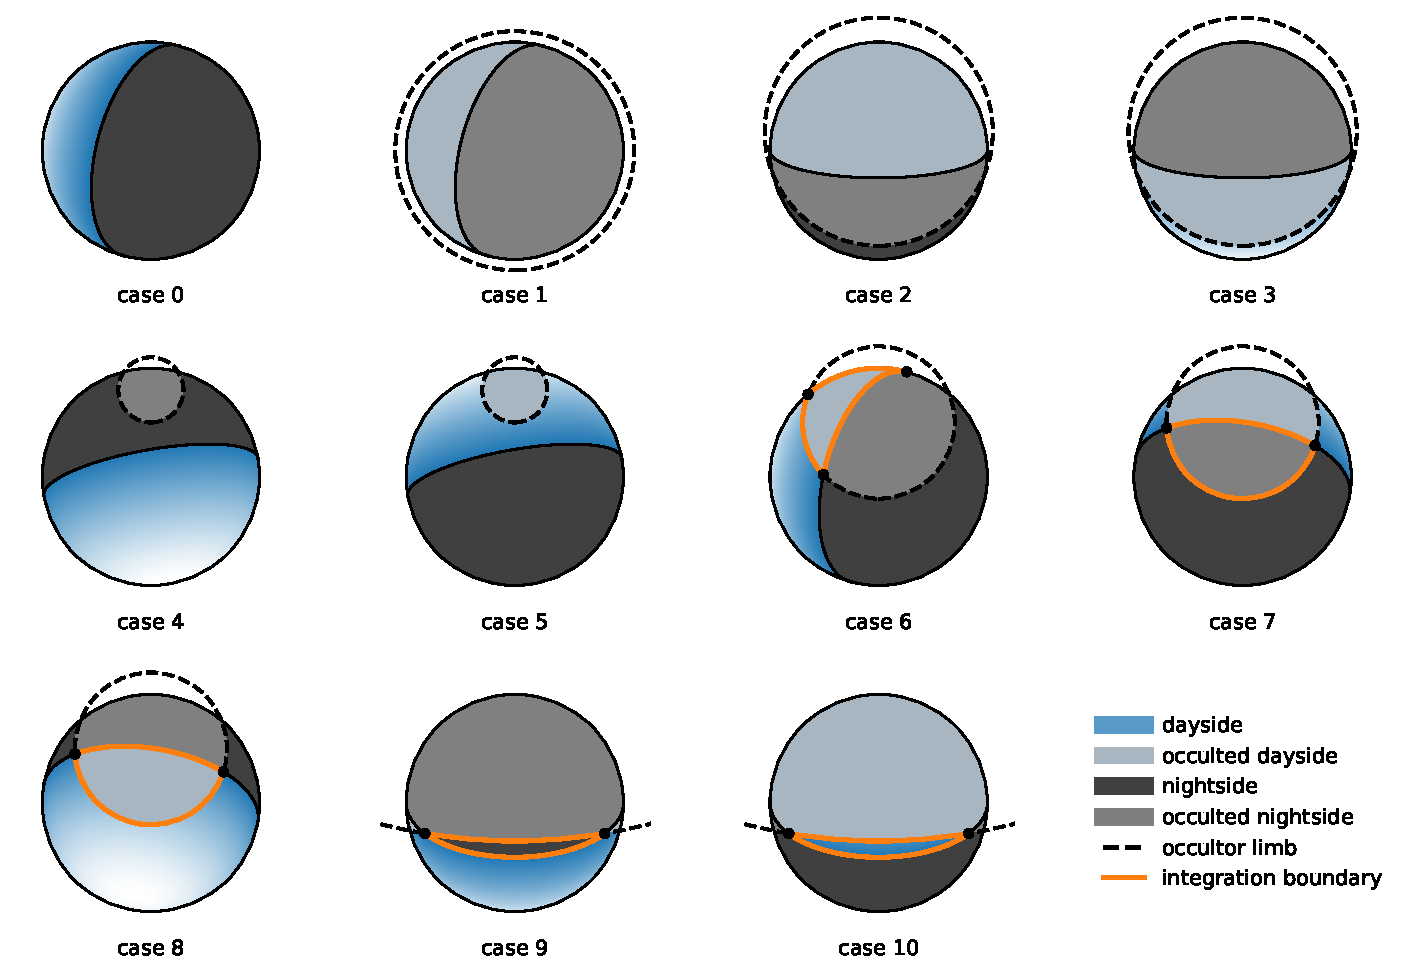
\includegraphics[width=\linewidth]{figures/cases.pdf}
        \oscaption{cases}{%
            The eight families of cases of occultations in reflected light.
            In these figures, the night side of the occulted body is colored
            black (dark grey if occulted), and the dayside is colored blue
            (light grey if occulted). The cases in the top row involve
            configurations in which the limb of the occultor does not intersect
            with the terminator at any point, so the visible flux may be
            computed in terms of classical \starry integrals. The remaining
            cases require integration along the red boundary (the curves
            $\mathcal{P}$, $\mathcal{T}$, and $\mathcal{Q}$ of
            \S\ref{sec:integration}), which
            include the terminator. These involve the evaluation of incomplete
            elliptic integrals and are derived below.
            \label{fig:cases}
        }
    \end{centering}
\end{figure}

\section{The Solution: Case 0}
\label{sec:cases-0}
%
Before we tackle configurations involving occultations, we must address the
simpler problem of computing the total visible flux from an unocculted
body in reflected light (see Figure~\ref{fig:illum}). This problem was
originally solved by \citet{Haggard2018} and subsequently adapted to the
\starry formalism in \citet{Luger2019b}, but for completeness we present
the detailed solution below.

Our task is to compute the solution vector for this
configuration, which we will denote $\bvec{s}^\top_0$.
Since in this case there is no occultor, it is
more convenient to perform the integration in a frame $\mathcal{F}''$ where the
semi-major axis of the terminator is aligned with the $x$-axis
(see Figure~\ref{fig:illum}); let us denote the matrix that rotates us
from $\mathcal{F}'$ to $\mathcal{F}''$ as $\bvec{R}''$.
It is also far easier to perform the integration
in the \emph{polynomial basis} $\tilde{\bvec{p}}$
\citep[Equation 7 in][]{Luger2019}:
%
\begin{align}
    \tilde{p}_{l,m}(x, y) & =
    \begin{dcases}
        x^\frac{\mu}{2} y^\frac{\nu}{2}
         & \qquad \mu, \nu \, \mathrm{even}
        \\[1em]
        x^\frac{\mu-1}{2} y^\frac{\nu-1}{2} z(x, y)
         & \qquad \mathrm{otherwise} \quad,
    \end{dcases}
\end{align}
%
where $\tilde{\bvec{p}}$ is again ordered such that the component at
index $n$ is $\tilde{p}_{l,m}$, with $l$ and $m$ given by
Equation~(\ref{eq:lm}).
Now, if $\bvec{r}^\top$ is the solution to the surface integrals in the
polynomial basis in $\mathcal{F}''$,
we may compute the desired solution vector in the Green's basis from
%
\begin{align}
    \label{eq:sTref}
    \bvec{s}^\top_0 & = \bvec{r}^\top \bvec{A_1} \bvec{R}'' \bvec{A}^{-1}
    \quad,
\end{align}
%
where $\bvec{A_1}$ \citep[Equation B11 in][]{Luger2019}
transforms the solution into the spherical harmonic basis so it can
be rotated out of the integration frame $\mathcal{F}''$ via $\bvec{R}''$, and
$\bvec{A}^{-1}$ \citep[Equation B13 in][]{Luger2019} transforms the
result into the Green's basis (in which $\bvec{s}^\top$ is defined).

Our task is thus to compute $\bvec{r}^\top$.
In frame $\mathcal{F}''$, the body sits at the origin and is
illuminated by a point source in the
$y-z$ plane at coordinates $(0, y_s, z_s)$ as in Figure~\ref{fig:illum}.
The day/night terminator is a half-ellipse whose semi-major axis
is unity and is aligned with the $x$-axis. The semi-minor axis is given
by $b = -\nicefrac{z_s}{\sqrt{y_s^2 + z_s^2}}$, where $b > 0$ corresponds to
a half-ellipse that is concave down and $b < 0$ to one that is concave up.
It is straightforward to show
that the illumination at a point $(x, y)$ on the projected disk is
given by
%
\begin{proof}{illum}
    \Psi(b; x, y) & =
    \begin{dcases}
        b_cy - bz(x, y) &
        \quad\quad\quad\quad\quad\quad\quad\quad\quad\quad
        y \geq b \sqrt{1 - x^2}
        \\
        0               &
        \quad\quad\quad\quad\quad\quad\quad\quad\quad\quad
        \mathrm{otherwise}
    \end{dcases}
    \quad ,
    \label{eq:illum}
\end{proof}
%
where $b_c = \sqrt{1 - b^2}$.
%
The elements of the solution vector may then be computed from
%
\begin{align}
    \label{eq:rT}
    r_{l, m}(b) & =
    \int_{-1}^{1}
    \int_{b\sqrt{1 - x^2}}^{\sqrt{1 - x^2}}
    \tilde{p}_{n(\mu,\nu)}(x, y)
    \Psi(b; x, y)
    \ \dd y \ \dd x
    \quad.
\end{align}
%
This is the integral of the illumination-weighted intensity of each
term in the polynomial basis over the projected visible dayside of the
body.
%
Equation~(\ref{eq:rT}) may be solved analytically in terms of purely
trigonometric and algebraic functions of $b$:
%
\begin{proof}{rT}
    \label{eq:rTsoln}
    r_{l, m}(b) & =
    \begin{cases}
        \frac{b_c\left(1 - b^{\frac{\nu + 4}{2}}\right)}{2}
        J_{\frac{\mu}{2}, \frac{\nu + 2}{2}} -
        b I_\frac{\nu}{2}(b) K_{\frac{\mu}{2}, \frac{\nu}{2}}
        %
         &
        %
        \qquad
        \mu, \nu \ \mathrm{even}
        %
        \\[1em]
        %
        b_c
        I_{\frac{\nu + 1}{2}}(b) K_{\frac{\mu - 1}{2}, \frac{\nu + 1}{2}}
        %
        \\[0.5em]
        \qquad
        %
        - \frac{b}{2} \bigg\{
        \left(1 - b^{\frac{\nu + 1}{2}}\right)
        \left(
        J_{\frac{\mu - 1}{2}, \frac{\nu - 1}{2}} -
        J_{\frac{\mu + 3}{2}, \frac{\nu - 1}{2}}
        \right)
        \\[0.5em]
        \qquad\qquad
        -
        \left(1 - b^{\frac{\nu + 5}{2}}\right)
        J_{\frac{\mu - 1}{2}, \frac{\nu + 3}{2}}
        \bigg\}
        %
         &
        %
        \qquad
        \mathrm{otherwise}
        %
    \end{cases}
\end{proof}
%
where
%
\begin{proof}{rT}
    \label{eq:IJK}
    I_{j}(b) &= \int_b^1 a^j \sqrt{1 - a^2} \dd a
    \nonumber \\
    %
    J_{i,j} &=
    \frac{
        \Gamma\left(\frac{i + 1}{2}\right)
        \Gamma\left(\frac{j + 1}{2}\right)
    }
    {
        \Gamma\left(\frac{i + j + 4}{2}\right)
    }
    %
    \nonumber \\
    %
    K_{i,j} &=
    \frac{
        \Gamma\left(\frac{i + 1}{2}\right)
        \Gamma\left(\frac{j + 4}{2}\right)
    }
    {
        \Gamma\left(\frac{i + j + 5}{2}\right)
    }
    \quad.
\end{proof}
%
Given initial conditions
%
\\[1em]
\begin{minipage}{.33\linewidth}
    \begin{proof}{rT}
        I_{0}(b) &= \frac{\arccos(b) - bb_c}{2}
        %
        \nonumber \\
        %
        I_{1}(b) &= \frac{b_c^3}{3}
        %
        \nonumber
    \end{proof}
\end{minipage}%
\begin{minipage}{.32\linewidth}
    \begin{proof}{rT}
        J_{0,0} &= \pi
        %
        \nonumber \\
        %
        J_{0,1} &= \frac{4}{3}
        %
        \nonumber
    \end{proof}
\end{minipage}%
\begin{minipage}{.33\linewidth}
    \begin{proof}{rT}
        \label{eq:IJK0}
        K_{0,0} &= \frac{4}{3}
        %
        \nonumber \\
        K_{0,1} &= \frac{3\pi}{8}
    \end{proof}
\end{minipage}
\\[1em]
%
we may compute all higher order terms from the recurrence relations
%
\begin{proof}{rT}
    \label{eq:IJKrec}
    I_{j}(b) &= \frac{b^n b_c^3 + (j - 1) I_{j - 2}(b)}{j + 2}
    %
    \nonumber \\
    %
    J_{0,j} &= \left(\frac{j - 1}{j + 2}\right) J_{0,j-2}
    %
    \nonumber \\
    %
    K_{0,j} &= \left(\frac{j + 2}{j + 3}\right) K_{0,j-2}
    %
    \nonumber \\
    %
    J_{i,j} &= \left(\frac{i - 1}{i + j + 2}\right) J_{i-2,j}
    %
    \nonumber \\
    %
    K_{i,j} &= \left(\frac{i - 1}{i + j + 3}\right) K_{i-2,j}
    \quad.
\end{proof}
%


\section{The Solution: Cases 1--4}
\label{sec:cases-1-4}
Cases 1--4 (see Figure~\ref{fig:cases}) involve configurations in which the
occultor does not intersect with
the terminator of the occulted body, and are therefore significantly easier to
solve.

\section{The Solution: Cases 5--8}
\label{sec:cases-5-8}
Cases 5--8 (see Figure~\ref{fig:cases}).

\begin{figure}[t!]
    \begin{centering}
        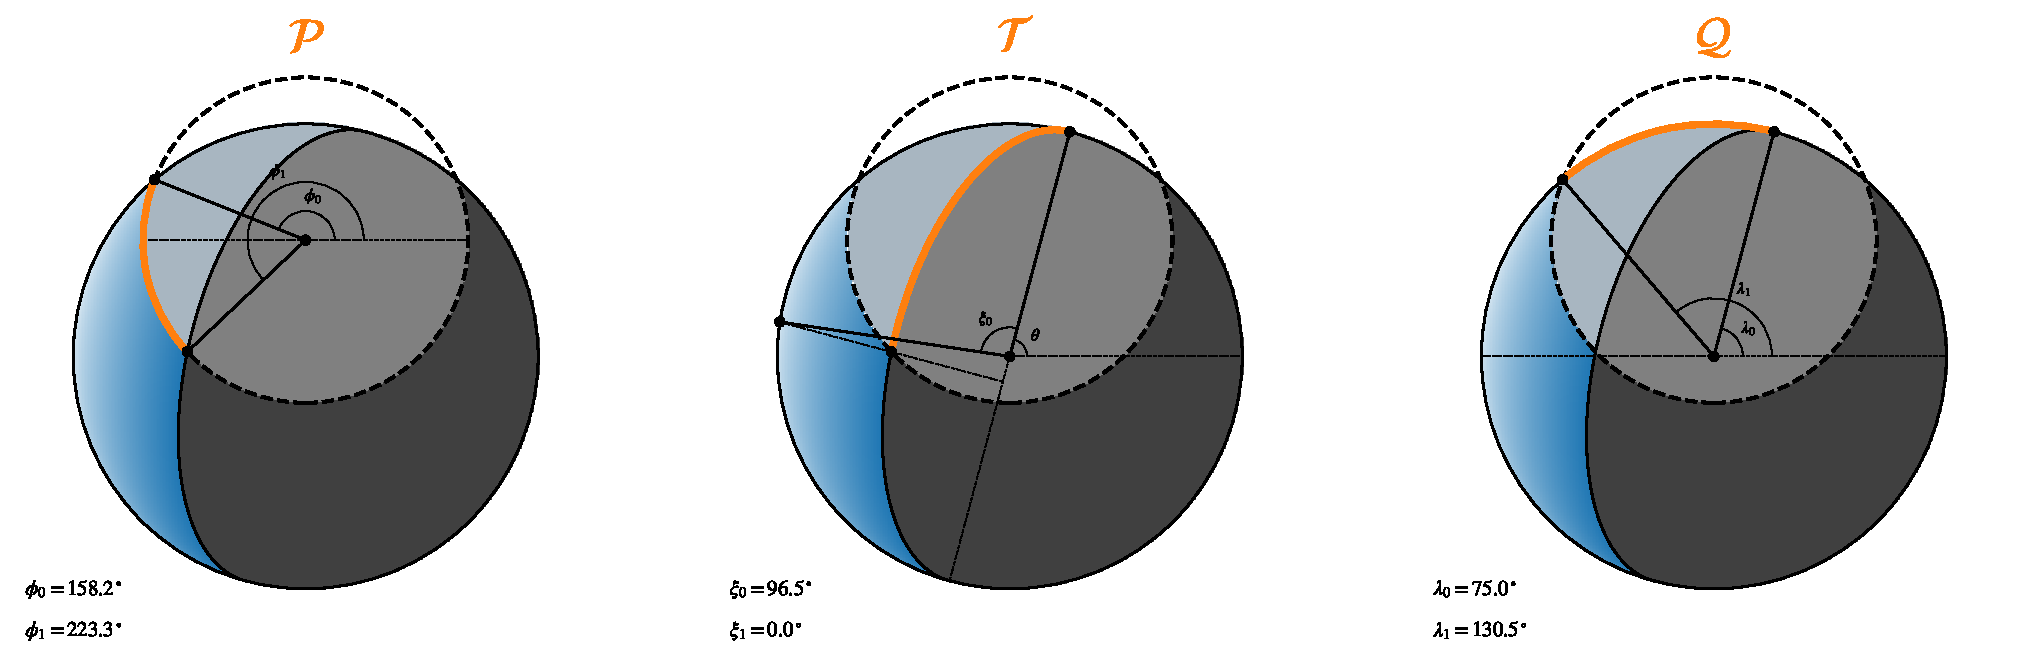
\includegraphics[width=\linewidth]{figures/geometry.pdf}
        \oscaption{geometry}{%
            Geometry of an occultation in reflected light, corresponding
            to case 5 in Figure~\ref{fig:cases}. The surface integral over
            the blue region is computed from the antiderivatives of the
            surface intensity map counter-clockwise along the boundary curves
            $\mathcal{P}$, $\mathcal{T}$, and $\mathcal{Q}$.
            \label{fig:geometry}
        }
    \end{centering}
\end{figure}

As in \citet{Luger2019}, the elements of the solution vector $\mathbf{s}^\top$
are given by the line integral
%
\begin{align}
    \label{eq:s}
    s_{n(\mu,\nu)} = \oint \mathbf{G}_{\mu,\nu} \cdot \dd\mathbf{r}
\end{align}
%
where
%
\begin{align}
    \label{eq:G}
    \bvec{G}_{\mu,\nu} (x, y) & =
    \begin{dcases}
        %
        x^{\frac{\mu + 2}{2}}
        y^{\frac{\nu}{2}}
        \,\yhat
         & \qquad \mu, \nu \, \mathrm{even}
        \\[1em]
        %
        \frac{1-z(x, y)^3}{3(1-z(x, y)^2)}\bigg(-y \, \xhat + x \, \yhat\bigg)
         & \qquad \mu = \nu = 1
        \\[1em]
        %
        x^{l-2}
        z(x, y)^3
        \,\xhat
         & \qquad \nu \, \mathrm{odd}, \,
        \mu = 1, \,
        \frac{\mu + \nu}{2} \, \mathrm{even}
        \\[1em]
        %
        x^{l-3}
        y
        z(x, y)^3
        \,\xhat
         & \qquad \nu \, \mathrm{odd}, \,
        \mu = 1, \,
        \frac{\mu + \nu}{2} \, \mathrm{odd}
        \\[1em]
        %
        x^{\frac{\mu-3}{2}}
        y^{\frac{\nu-1}{2}}
        z(x, y)^3
        \,\yhat
         & \qquad \mathrm{otherwise,}
    \end{dcases}
\end{align}
%
and
%
\begin{align}
    \dd \bvec{r} & = -r \sin\varphi \, \dd \varphi \, \xhat +
    r \cos\varphi \, \dd \varphi \, \yhat
    \quad,
\end{align}
%
where $\varphi = \varphi(x, y)$ is the parametrized angle along the
arc of integration. Generally, there are at most three arcs bounding a given
closed surface of integration, which we will denote $\mathcal{P}$,
$\mathcal{Q}$, and $\mathcal{T}$. These are shown for a typical occultor-occulted
configuration in Figure~\ref{fig:geometry}.


\section{Performance}
\label{sec:performance}

%
\begin{figure}[h!]
    \begin{centering}
        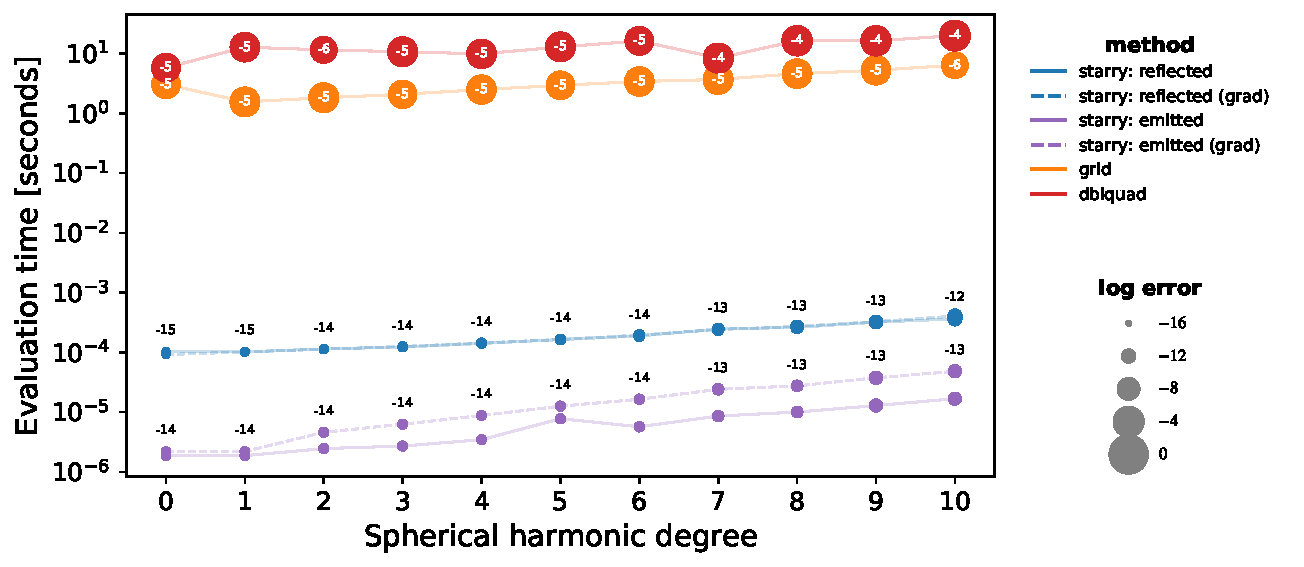
\includegraphics[width=\linewidth]{figures/speed.pdf}
        \oscaption{speed}{%
            Evaluation time for the starry algorithm.
            \label{fig:speed}
        }
    \end{centering}
\end{figure}


\section{Integration}
\label{sec:integration}

\subsection{Definitions}
%
Define the pairwise difference operator
%
\begin{align}
    \label{eq:pairdiff}
    \Delta \boldsymbol{v} \equiv \sum_{i=0}^{\frac{N - 1}{2}}
    \left( v_{2i + 1} - v_{2i} \right)
\end{align}
%
which sums the difference of successive pairs of values in
an array $\boldsymbol{v} = \{ v_0, v_1, v_2, v_3, {\cdot\cdot\cdot}, v_N\}$.

Define the quantity
%
\begin{align}
    \label{eq:q}
    \boldsymbol{q}(k^2, \bkappa) = \sqrt{1 - \frac{\sinhalfkap[2]}{k^2}}
    \quad.
\end{align}

\subsection{$\mathcal{H}_{u,v}$}
%
The function $\mathcal{H}_{u,v}$ is given by
%
\begin{align}
    \label{eq:H}
    \mathcal{H}_{u,v}(\blambda) & =
    \lamint{
        \cos^u\varphi
        \sin^v\varphi
    }
    \quad.
\end{align}
%
The integral in this expression is the same as that in Equation (D27)
of \citet{Luger2019}, except for a change in the limits of integration.
We can compute this integral recursively given four lower boundary conditions:
%
\begin{proof}{H}
    \label{eq:Hlower}
    \mathcal{H}_{0,0}(\blambda) &= \Delta \blambda
    %
    \nonumber \\
    %
    \mathcal{H}_{1,0}(\blambda) &= \Delta \sin\blambda
    %
    \nonumber \\
    %
    \mathcal{H}_{0,1}(\blambda) &= -\Delta \cos\blambda
    %
    \nonumber \\
    %
    \mathcal{H}_{1,1}(\blambda) &= -\frac{\Delta\cos^2\blambda}{2}
    %
    \quad.
\end{proof}
%
The remaining terms may be computed by upward recursion using the
relations
%
\begin{proof}{H}
    \label{eq:Hrec1}
    \mathcal{H}_{u,v}(\blambda) &=
    \frac{
        -\Delta \left(
        \cos^{u + 1} \blambda
        \sin^{v - 1} \blambda
        \right)
        +(v - 1)\mathcal{H}_{u,v - 2}(\blambda)
    }{u + v}
\end{proof}
%
for $u < 2, v \ge 2$ and
%
\begin{proof}{H}
    \label{eq:Hrec2}
    \mathcal{H}_{u,v}(\blambda) &=
    \frac{
        \Delta \left(
        \cos^{u - 1} \blambda
        \sin^{v + 1} \blambda
        \right)
        + (u - 1)\mathcal{H}_{u - 2,v}(\blambda)
    }{u + v}
\end{proof}
%
for all remaining terms.

\subsection{$\mathcal{T}_{2}$}
%
The function $\mathcal{T}_{2}$ is given by
%
\begin{align}
    \label{eq:T2}
    \mathcal{T}_{2}(b, \bxi) & = ?
    \quad.
\end{align}

\begin{proof}{T2}
    \mathcal{T}_{2}(b, \bxi) &= -\sgn(b) \Delta \boldsymbol{f}(b, \bxi)
\end{proof}
%
where
%
\begin{proof}{T2}
    \begin{split}
        f_i(b, \xi_i) =
        \frac{1}{3}\scalebox{1.4}{\Bigg(}
        &\arctan\left( \frac{|b|\sin\xi_i}{\cos\xi_i} \right)
        %
        \\
        %
        &- \sgn\left({\sin\xi_i}\right)
        \left(
        \arctan
        \left(
            \frac{
                \left(\frac{\sin\xi_i}{1 + \cos\xi_i}\right)^2 + 2 b^2 - 1
            }{2 |b| \sqrt{1 - b^2}}
            \right)
        + |b| \sqrt{1 - b^2} \cos\xi_i
        \right)
        %
        \\
        %
        &+ \phi(b, \xi_i)
        \scalebox{1.4}{\Bigg)}
    \end{split}
\end{proof}
%
and
%
\begin{proof}{T2}
    \phi(b, \xi_i) & =
    \begin{cases}
        0                          & \qquad 0 \leq \xi_i < \frac{\pi}{2}     \\
        \pi                        & \qquad \frac{\pi}{2} \leq \xi_i < \pi   \\
        2 |b| \sqrt{1 - b^2}       & \qquad \pi < \xi_i \leq \frac{3\pi}{2}  \\
        \pi + 2 |b| \sqrt{1 - b^2} & \qquad \frac{3\pi}{2} \leq \xi_i < 2\pi
        \quad.
    \end{cases}
\end{proof}

\subsection{$\mathcal{U}_v$}
%
The function $\mathcal{U}_v$ is given by
%
\begin{align}
    \label{eq:U}
    \mathcal{U}_v(\bkappa) =
    \kapint{\cos\varphi\sin^{2v}\varphi}
    \quad.
\end{align}
%
This integral has an analytic solution for all $v$:
%
\begin{proof}{U}
    \label{eq:Usol}
    \mathcal{U}_v(\bkappa) &= \frac{\Delta \sinhalfkap[v+1]}{v + 1}
    \quad.
\end{proof}
%

\subsection{$\mathcal{I}_v$}
%
The function $\mathcal{I}_v$ is given by
%
\begin{align}
    \label{eq:I}
    \mathcal{I}_v(\bkappa) & =
    \kapint{\sinhalfkap[2v]}
    \quad.
\end{align}
%
The integral in this expression is the same as that in Equation (D38)
of \citet{Luger2019}, except for a change in the limits of integration.
As in \citet{Luger2019}, we can compute this integral recursively given
a trivial lower boundary condition:
%
\begin{proof}{I}
    \label{eq:Irec}
    \mathcal{I}_0(\bkappa) &=
    \frac{\Delta \bkappa}{2}
    %
    \nonumber \\
    %
    \mathcal{I}_v(\bkappa) &=
    \frac{1}{2v}
    \bigg(
    (2v - 1) \mathcal{I}_{v-1}(\bkappa) -
    \Delta \left(\sinhalfkap[2v - 1]\coshalfkap\right)
    \bigg)
\end{proof}
%
where the last expression is valid for all $v > 0$. We find that this algorithm
is generally stable, except when $\sin\left(\frac{\bkappa}{2}\right)$ is small. In
that limit, we evaluate $\mathcal{I}_N(\bkappa)$ by numerical integration of
Equation~(\ref{eq:I}) using Gauss-Legendre quadrature with \STARRYQUADPOINTS
points. We then recurse downward by substituting $v \rightarrow v + 1$ in
Equation~(\ref{eq:Irec}) and solving for $\mathcal{I}_v(\bkappa)$.

\subsection{$\mathcal{J}_v$}
%
The function $\mathcal{J}_v$ is given by
%
\begin{align}
    \label{eq:J}
    \mathcal{J}_v(k^2, \bkappa) =
    \kapint{
        \sin^{2v}\varphi
        \left(1 - \frac{\sin^2\varphi}{k^2}\right)^\frac{3}{2}
    }
    \quad.
\end{align}
%
The integral in this expression is again the same as that in Equation (D39)
of \citet{Luger2019}, except for a change in the limits of integration.
In that paper, we computed all terms
$\{ \mathcal{J}_0, {\cdot\cdot\cdot}, \mathcal{J}_\vmax \}$ from a three-term
recurrence relation and two boundary conditions. In the case of upward
recursion, the boundary conditions $\mathcal{J}_0$ and $\mathcal{J}_1$ were
computed analytically from the complete elliptic integrals $K(k^2)$
and $E(k^2)$. In cases where upward recursion was not numerically stable, we
evaluated $\mathcal{J}_\vmax$ and $\mathcal{J}_{\vmax-1}$
via a quickly convergent series expansion and recursed downward.

In order to solve Equation~(\ref{eq:J}), it is possible to
replace the complete elliptic integrals $K(k^2)$ and $E(k^2)$ in the lower
boundary conditions \citep[Equation D46 in ][]{Luger2019} with the
incomplete elliptic integrals $F(k^2, \kappa)$ and $E(k^2, \kappa)$,
then use the same upward
recursion relation to obtain analytic solutions for all $\mathcal{J}_v$:
%
\begin{proof}{J}
    \label{eq:Jrec}
    \mathcal{J}_0(k^2, \bkappa) &=
    \frac{1}{3} \bigg(
    2 \left(2 - \frac{1}{k^2}\right) \DE +
    \left(\frac{1}{k^2} - 1\right) \DF +
    \Delta \boldsymbol{z}_0(k^2, \bkappa)
    \bigg)
    %
    \nonumber \\
    %
    \mathcal{J}_1(k^2, \bkappa) &=
    \frac{1}{15} \bigg(
    \left(-3 k^2 + 13 - \frac{8}{k^2}\right) \DE +
    \left(3 k^2 - 7 + \frac{4}{k^2}\right) \DF +
    \Delta \boldsymbol{z}_1(k^2, \bkappa)
    \bigg)
    %
    \nonumber \\
    %
    \mathcal{J}_v(k^2, \bkappa) &=
    \frac{1}{2v + 3}
    \bigg(
    2 \left( v + 1 + (v - 1) k^2 \right) \mathcal{J}_{v - 1} -
    (2v - 3) k^2 \mathcal{J}_{v - 2}
    + \Delta \boldsymbol{z}_v(k^2, \bkappa)
    \bigg)
\end{proof}
%
%
where the last expression is valid for all $v > 1$ and
%
\begin{proof}{J}
    \label{eq:Jrec_z}
    \boldsymbol{z}_0(k^2, \boldsymbol{\kappa}) & =
    \frac{
        \sinhalfkap
        \coshalfkap
        \boldsymbol{q}(k^2, \bkappa)
    }{
        k^2
    }
    %
    \nonumber\\
    %
    \boldsymbol{z}_1(k^2, \boldsymbol{\kappa}) & =
    \left(\left(3 \sinhalfkap[2] + 4\right) - 6k^2\right)
    \boldsymbol{z}_0(k^2, \boldsymbol{\kappa})
    %
    \nonumber\\
    %
    \boldsymbol{z}_v(k^2, \boldsymbol{\kappa}) & =
    k^2
    \sinhalfkap[2v - 3]
    \coshalfkap
    \boldsymbol{q}(k^2, \boldsymbol{\kappa})^5
    \quad.
\end{proof}
%
However, in practice we find that this procedure is even more numerically
unstable than it was in \citet{Luger2019}.
To address this, we express the recurrence structure of the problem as
a tridiagonal system with one lower boundary condition $\mathcal{J}_0$
and one upper boundary condition $\mathcal{J}_\vmax$:
%
\begin{proof}{J}
    \label{eq:Jtri}
    \begin{pmatrix}
        a_0 & 1   &     &        &         &         \\
        b_1 & a_1 & 1   &        &         &         \\
            & b_2 & a_2 & 1      &         &         \\
            &     & b_0 & a_3    & 1       &         \\
            &     &     & \ddots & \ddots  & \ddots  \\
            &     &     &        & b_\vmax & a_\vmax
    \end{pmatrix}
    \begin{pmatrix}
        \mathcal{J}_1   \\
        \mathcal{J}_2   \\
        \mathcal{J}_3   \\
        \mathcal{J}_4   \\
        \cdot\cdot\cdot \\
        \mathcal{J}_{\vmax-1}
    \end{pmatrix}
    =
    \begin{pmatrix}
        c_0 - b_0 \mathcal{J}_0 \\
        c_1                     \\
        c_2                     \\
        c_3                     \\
        \cdot\cdot\cdot         \\
        c_\vmax - \mathcal{J}_\vmax
    \end{pmatrix}
\end{proof}
%
where the recursion coefficients are given by
%
\begin{proof}{J}
    \label{eq:Jtri_coeffs}
    a_v(k) &= -2\frac{(v + 1) + (v - 1) k^2}{2v + 3} \nonumber \\
    b_v(k) &= \frac{(2v - 3) k^2}{2v + 3} \nonumber \\
    c_v(k^2, \bkappa) &= \Delta
    \bigg(
    \frac{
            \boldsymbol{z}_v(k^2, \boldsymbol{\kappa})
        }{
            2v + 3
        }
    \bigg)
    \quad.
\end{proof}
%
Solving this matrix system yields values for all
intermediate $\{ \mathcal{J}_1, {\cdot\cdot\cdot}, \mathcal{J}_{\vmax - 1} \}$.
While efficient algorithms exist for solving tridiagonal problems, we obtain
far better numerical stability by instead performing traditional LU
decomposition. We find that this algorithm is stable in all the regimes that we
tested.

We evaluate the upper boundary condition $\mathcal{J}_{\vmax}$ by numerical
integration of Equation~(\ref{eq:J}) via Gauss-Legendre quadrature with
\STARRYQUADPOINTS points. While the lower boundary condition may be computed
analytically from Equation~(\ref{eq:Jrec}),
in practice we achieve better precision via numerical
integration (as above), with negligible effects on computational performance.

\subsection{$\mathcal{W}_n$}
%
The function $\mathcal{W}_n$ is given by
%
\begin{align}
    \label{eq:W}
    % TODO
    \mathcal{W}_n = \int
\end{align}
%
This integral has a closed-form solution:
%
\begin{align}
    \label{eq:Wsol}
    \mathcal{W}_n =
    \frac{\sin^{2n + 2}\left(\frac{\bkappa}{2}\right)}{2n + 5}
    \left(
    \frac{3}{n+1}
        {_2F_1}\left(-\frac{1}{2}, n + 1; n + 2; 1 - q^2\right) + 2 q^3
    \right)
\end{align}
%
where ${_2F_1}(a, b; c; z)$ is the Gauss hypergeometric function.


% by either upward recursion (stable for |1 - q^2| > 1/2) or downward
% recursion (always stable).

% Bibliography
\bibliography{bib}


\end{document}
